\documentclass{article}
\usepackage[utf8]{inputenc}
\usepackage{amsmath}
\usepackage{amsfonts}
\usepackage{mathrsfs}
\usepackage{graphicx}
\usepackage[top=30truemm,bottom=30truemm,left=30truemm,right=30truemm]{geometry}


\title{Chaotic Dynamics: Homework 2}
\author{Kansuke Ikehara (Kansuke.Ikehara@colorado.edu)}

\begin{document}
\maketitle

\subsection*{Problem 1}

\begin{figure}[hb]
	\centering
	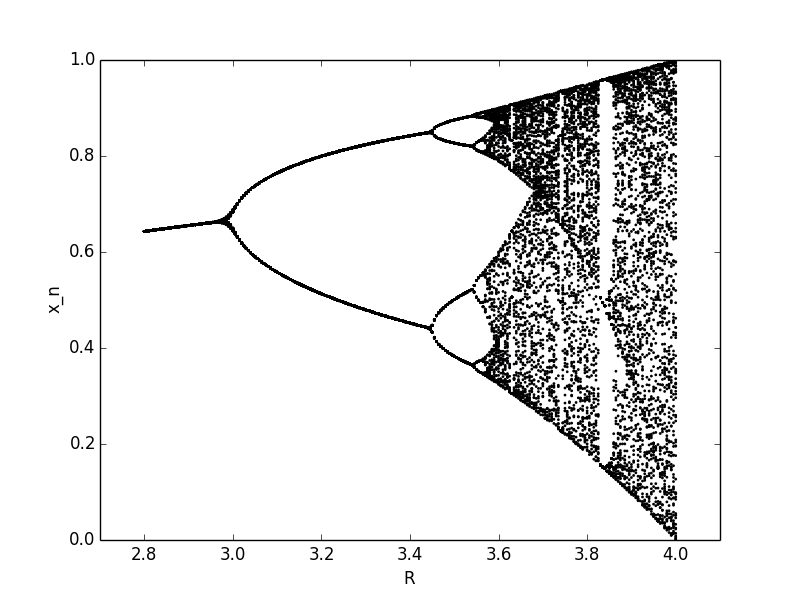
\includegraphics[height=2in]{figs/fig1.png}
	\caption{Bifurcation plot of logistic map}
	\label{BifLog}
\end{figure}

Fig.\ref{BifLog} shows a bifurcation plot of logistic map. The interval between the value $R$ is $0.01$.

\subsection*{Problem 2}
In this problem, I used a zooming functionality of matplotlib, a Python's scientific graphics library, in order to see the bifurcation points, therefore not gained the best in terms of accuracy. It is, however, good enough to see the trend going on in the sequence. The sequence of $\delta$s is as follows:
\[
	\delta_{1} = \frac{3 - 0}{3.446 - 3} \approx 6.726
\]
\[
	\delta_{2} = \frac{3.446 - 3}{3.543 - 3.446} \approx 4.598
\]
\[
	\delta_{3} = \frac{3.543 - 3.446}{3.564 - 3.543} \approx 4.619
\]
As you can see it gradually gets closer to the true value $4.66..$ .

\subsection*{Problem 3}
Fig.\ref{Henon} shows the bifurcation plot of H\'enon map. The sequence of $\delta$s is as follows:
\[
	\delta_{1} = \frac{0.351 - 0}{0.905 - 0.351} \approx 0.6336
\]
\[
	\delta_{2} = \frac{0.905 - 0.351}{1.0225 - 0.905} \approx 4.7149
\]
\[
	\delta_{3} = \frac{1.0225 - 0.905}{1.0512 - 1.0225} \approx 4.0941
\]

$\delta_{3}$ is actually a bit deviating from the value $4.66..$, but this could be due to the accuracy of measuring bifurcation points from the plot itself. 

\begin{figure}[hb]
	\centering
	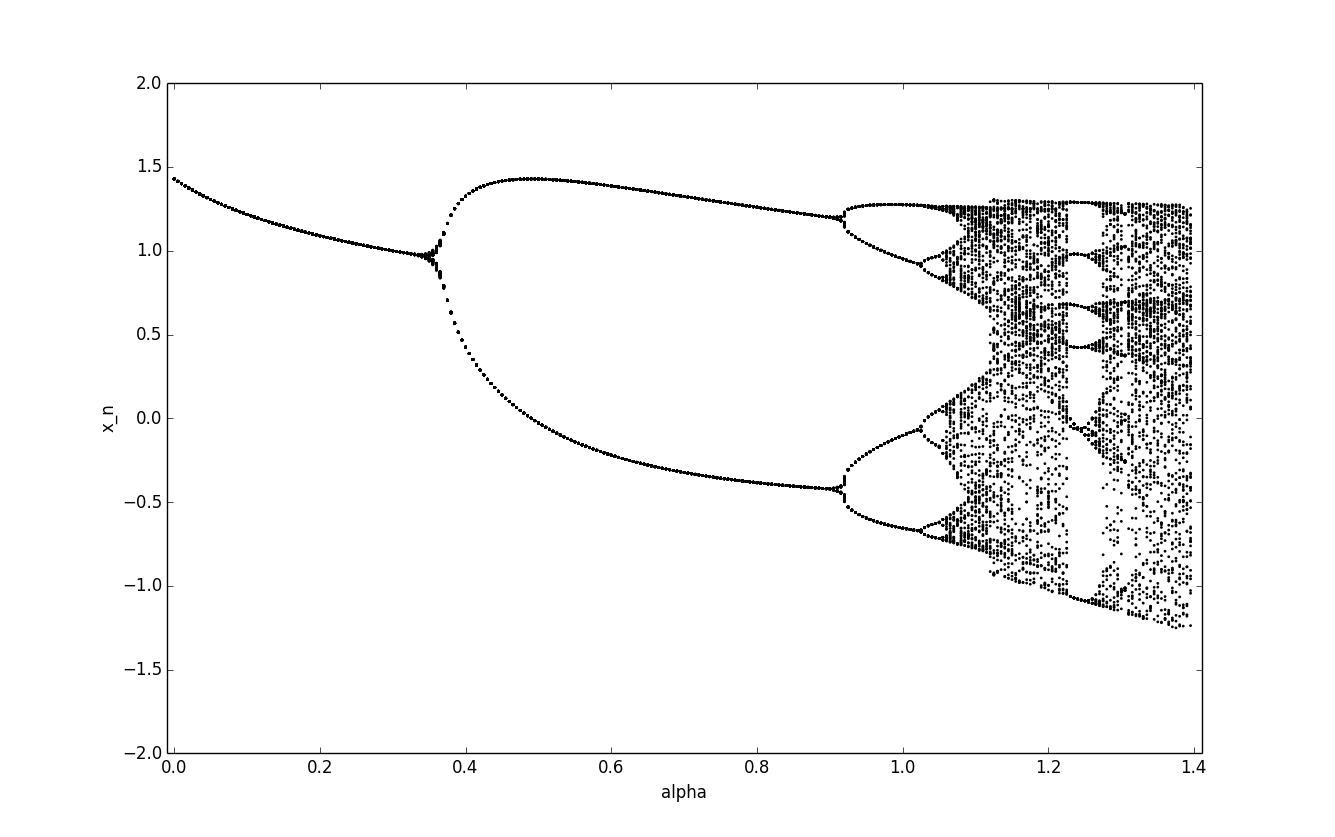
\includegraphics[height=2in]{figs/fig3.png}
	\caption{Bifurcation plot of H\'enon map}
	\label{Henon}
\end{figure}

\subsection*{Problem 4}
Fig.\ref{3} shows a plot of $x_{n+1}$ versus $x_{n}$ of H\'enon map. As we can see the plot is \textit{unimodal}, meaning that its shape is smooth-curved and it has only one maximum. As stated in \textit{Storogatz Chapter 10.6} The number $\delta$ converges to 4.66.. if the map is unimodal. Since H\'enon map is a kind of unimodal map, its $\delta$ should also converge to the value 4.66.. Therefore, the answers to problems 2 and 3 should be the same.
\begin{figure}[hb]
	\centering
	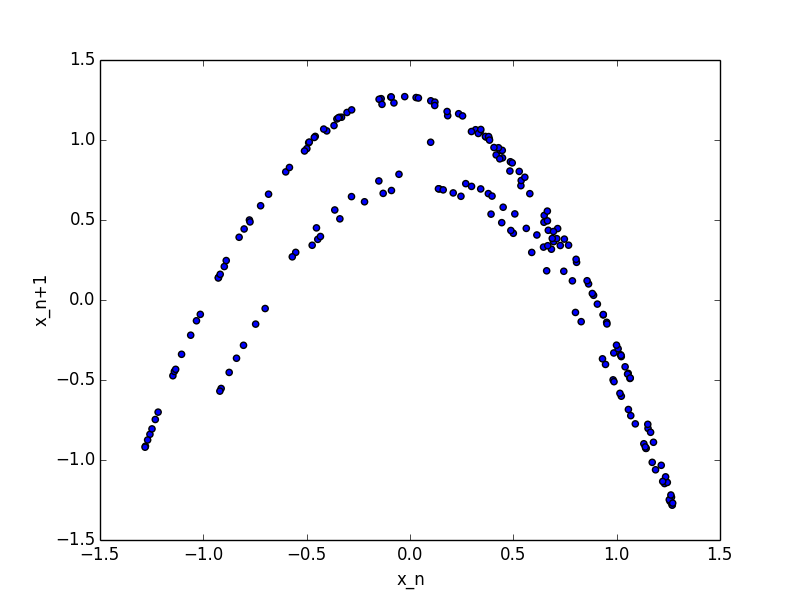
\includegraphics[height=2in]{figs/fig4.png}
	\caption{$x_{n+1}$ vs. $x_{n}$ of H\'enon map}
	\label{3}
\end{figure}

\end{document}












